% Created by tikzDevice version 0.12.6 on 2026-10-30 11:40:31
% !TEX encoding = UTF-8 Unicode
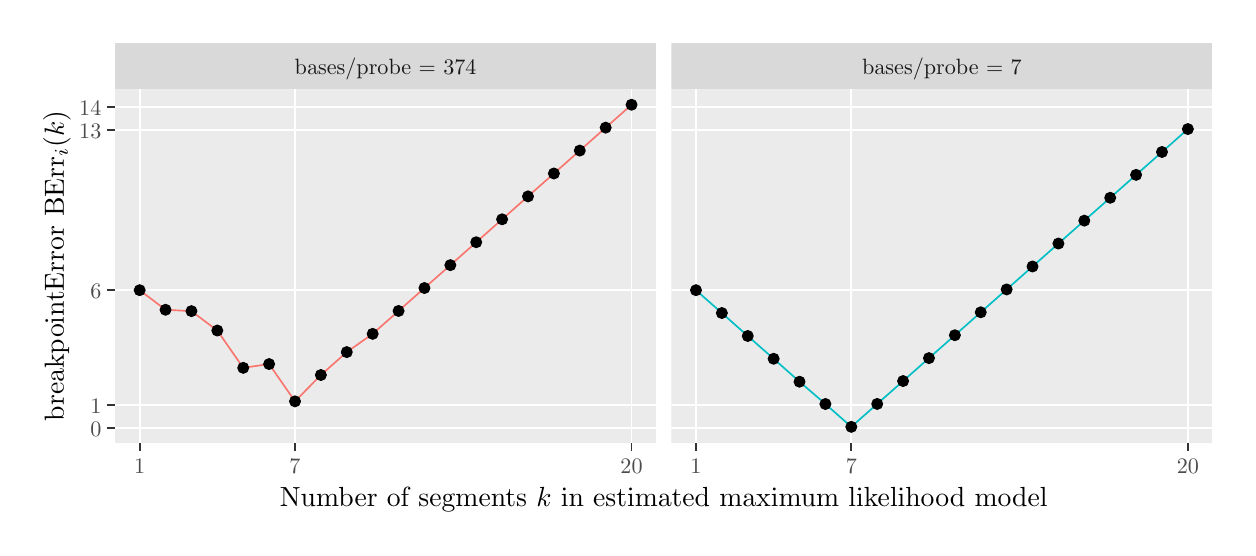
\begin{tikzpicture}[x=1pt,y=1pt]
\definecolor{fillColor}{RGB}{255,255,255}
\path[use as bounding box,fill=fillColor,fill opacity=0.00] (0,0) rectangle (433.62,180.67);
\begin{scope}
\path[clip] (  0.00,  0.00) rectangle (433.62,180.67);
\definecolor{drawColor}{RGB}{255,255,255}
\definecolor{fillColor}{RGB}{255,255,255}

\path[draw=drawColor,line width= 0.6pt,line join=round,line cap=round,fill=fillColor] (  0.00,  0.00) rectangle (433.62,180.68);
\end{scope}
\begin{scope}
\path[clip] ( 31.58, 30.61) rectangle (227.10,158.64);
\definecolor{fillColor}{gray}{0.92}

\path[fill=fillColor] ( 31.58, 30.61) rectangle (227.10,158.64);
\definecolor{drawColor}{RGB}{255,255,255}

\path[draw=drawColor,line width= 0.6pt,line join=round] ( 31.58, 36.13) --
	(227.10, 36.13);

\path[draw=drawColor,line width= 0.6pt,line join=round] ( 31.58, 44.41) --
	(227.10, 44.41);

\path[draw=drawColor,line width= 0.6pt,line join=round] ( 31.58, 85.81) --
	(227.10, 85.81);

\path[draw=drawColor,line width= 0.6pt,line join=round] ( 31.58,143.76) --
	(227.10,143.76);

\path[draw=drawColor,line width= 0.6pt,line join=round] ( 31.58,152.04) --
	(227.10,152.04);

\path[draw=drawColor,line width= 0.6pt,line join=round] ( 40.47, 30.61) --
	( 40.47,158.64);

\path[draw=drawColor,line width= 0.6pt,line join=round] ( 96.60, 30.61) --
	( 96.60,158.64);

\path[draw=drawColor,line width= 0.6pt,line join=round] (218.21, 30.61) --
	(218.21,158.64);
\definecolor{drawColor}{RGB}{248,118,109}

\path[draw=drawColor,line width= 0.6pt,line join=round] ( 40.47, 85.81) --
	( 49.82, 78.73) --
	( 59.18, 78.24) --
	( 68.53, 71.23) --
	( 77.89, 57.75) --
	( 87.24, 59.12) --
	( 96.60, 45.64) --
	(105.95, 55.16) --
	(115.31, 63.44) --
	(124.66, 70.03) --
	(134.02, 78.31) --
	(143.37, 86.59) --
	(152.73, 94.86) --
	(162.08,103.14) --
	(171.44,111.42) --
	(180.79,119.70) --
	(190.15,127.98) --
	(199.50,136.26) --
	(208.86,144.54) --
	(218.21,152.82);
\definecolor{drawColor}{RGB}{0,0,0}
\definecolor{fillColor}{RGB}{0,0,0}

\path[draw=drawColor,line width= 0.4pt,line join=round,line cap=round,fill=fillColor] ( 40.47, 85.81) circle (  1.96);

\path[draw=drawColor,line width= 0.4pt,line join=round,line cap=round,fill=fillColor] ( 49.82, 78.73) circle (  1.96);

\path[draw=drawColor,line width= 0.4pt,line join=round,line cap=round,fill=fillColor] ( 59.18, 78.24) circle (  1.96);

\path[draw=drawColor,line width= 0.4pt,line join=round,line cap=round,fill=fillColor] ( 68.53, 71.23) circle (  1.96);

\path[draw=drawColor,line width= 0.4pt,line join=round,line cap=round,fill=fillColor] ( 77.89, 57.75) circle (  1.96);

\path[draw=drawColor,line width= 0.4pt,line join=round,line cap=round,fill=fillColor] ( 87.24, 59.12) circle (  1.96);

\path[draw=drawColor,line width= 0.4pt,line join=round,line cap=round,fill=fillColor] ( 96.60, 45.64) circle (  1.96);

\path[draw=drawColor,line width= 0.4pt,line join=round,line cap=round,fill=fillColor] (105.95, 55.16) circle (  1.96);

\path[draw=drawColor,line width= 0.4pt,line join=round,line cap=round,fill=fillColor] (115.31, 63.44) circle (  1.96);

\path[draw=drawColor,line width= 0.4pt,line join=round,line cap=round,fill=fillColor] (124.66, 70.03) circle (  1.96);

\path[draw=drawColor,line width= 0.4pt,line join=round,line cap=round,fill=fillColor] (134.02, 78.31) circle (  1.96);

\path[draw=drawColor,line width= 0.4pt,line join=round,line cap=round,fill=fillColor] (143.37, 86.59) circle (  1.96);

\path[draw=drawColor,line width= 0.4pt,line join=round,line cap=round,fill=fillColor] (152.73, 94.86) circle (  1.96);

\path[draw=drawColor,line width= 0.4pt,line join=round,line cap=round,fill=fillColor] (162.08,103.14) circle (  1.96);

\path[draw=drawColor,line width= 0.4pt,line join=round,line cap=round,fill=fillColor] (171.44,111.42) circle (  1.96);

\path[draw=drawColor,line width= 0.4pt,line join=round,line cap=round,fill=fillColor] (180.79,119.70) circle (  1.96);

\path[draw=drawColor,line width= 0.4pt,line join=round,line cap=round,fill=fillColor] (190.15,127.98) circle (  1.96);

\path[draw=drawColor,line width= 0.4pt,line join=round,line cap=round,fill=fillColor] (199.50,136.26) circle (  1.96);

\path[draw=drawColor,line width= 0.4pt,line join=round,line cap=round,fill=fillColor] (208.86,144.54) circle (  1.96);

\path[draw=drawColor,line width= 0.4pt,line join=round,line cap=round,fill=fillColor] (218.21,152.82) circle (  1.96);
\end{scope}
\begin{scope}
\path[clip] (232.60, 30.61) rectangle (428.12,158.64);
\definecolor{fillColor}{gray}{0.92}

\path[fill=fillColor] (232.60, 30.61) rectangle (428.12,158.64);
\definecolor{drawColor}{RGB}{255,255,255}

\path[draw=drawColor,line width= 0.6pt,line join=round] (232.60, 36.13) --
	(428.12, 36.13);

\path[draw=drawColor,line width= 0.6pt,line join=round] (232.60, 44.41) --
	(428.12, 44.41);

\path[draw=drawColor,line width= 0.6pt,line join=round] (232.60, 85.81) --
	(428.12, 85.81);

\path[draw=drawColor,line width= 0.6pt,line join=round] (232.60,143.76) --
	(428.12,143.76);

\path[draw=drawColor,line width= 0.6pt,line join=round] (232.60,152.04) --
	(428.12,152.04);

\path[draw=drawColor,line width= 0.6pt,line join=round] (241.49, 30.61) --
	(241.49,158.64);

\path[draw=drawColor,line width= 0.6pt,line join=round] (297.62, 30.61) --
	(297.62,158.64);

\path[draw=drawColor,line width= 0.6pt,line join=round] (419.23, 30.61) --
	(419.23,158.64);
\definecolor{drawColor}{RGB}{0,191,196}

\path[draw=drawColor,line width= 0.6pt,line join=round] (241.49, 85.81) --
	(250.84, 77.56) --
	(260.20, 69.26) --
	(269.55, 61.03) --
	(278.91, 52.74) --
	(288.26, 44.68) --
	(297.62, 36.43) --
	(306.97, 44.71) --
	(316.33, 52.98) --
	(325.68, 61.26) --
	(335.04, 69.54) --
	(344.39, 77.82) --
	(353.75, 86.08) --
	(363.10, 94.38) --
	(372.46,102.66) --
	(381.81,110.94) --
	(391.17,119.20) --
	(400.52,127.48) --
	(409.88,135.75) --
	(419.23,144.03);
\definecolor{drawColor}{RGB}{0,0,0}
\definecolor{fillColor}{RGB}{0,0,0}

\path[draw=drawColor,line width= 0.4pt,line join=round,line cap=round,fill=fillColor] (241.49, 85.81) circle (  1.96);

\path[draw=drawColor,line width= 0.4pt,line join=round,line cap=round,fill=fillColor] (250.84, 77.56) circle (  1.96);

\path[draw=drawColor,line width= 0.4pt,line join=round,line cap=round,fill=fillColor] (260.20, 69.26) circle (  1.96);

\path[draw=drawColor,line width= 0.4pt,line join=round,line cap=round,fill=fillColor] (269.55, 61.03) circle (  1.96);

\path[draw=drawColor,line width= 0.4pt,line join=round,line cap=round,fill=fillColor] (278.91, 52.74) circle (  1.96);

\path[draw=drawColor,line width= 0.4pt,line join=round,line cap=round,fill=fillColor] (288.26, 44.68) circle (  1.96);

\path[draw=drawColor,line width= 0.4pt,line join=round,line cap=round,fill=fillColor] (297.62, 36.43) circle (  1.96);

\path[draw=drawColor,line width= 0.4pt,line join=round,line cap=round,fill=fillColor] (306.97, 44.71) circle (  1.96);

\path[draw=drawColor,line width= 0.4pt,line join=round,line cap=round,fill=fillColor] (316.33, 52.98) circle (  1.96);

\path[draw=drawColor,line width= 0.4pt,line join=round,line cap=round,fill=fillColor] (325.68, 61.26) circle (  1.96);

\path[draw=drawColor,line width= 0.4pt,line join=round,line cap=round,fill=fillColor] (335.04, 69.54) circle (  1.96);

\path[draw=drawColor,line width= 0.4pt,line join=round,line cap=round,fill=fillColor] (344.39, 77.82) circle (  1.96);

\path[draw=drawColor,line width= 0.4pt,line join=round,line cap=round,fill=fillColor] (353.75, 86.08) circle (  1.96);

\path[draw=drawColor,line width= 0.4pt,line join=round,line cap=round,fill=fillColor] (363.10, 94.38) circle (  1.96);

\path[draw=drawColor,line width= 0.4pt,line join=round,line cap=round,fill=fillColor] (372.46,102.66) circle (  1.96);

\path[draw=drawColor,line width= 0.4pt,line join=round,line cap=round,fill=fillColor] (381.81,110.94) circle (  1.96);

\path[draw=drawColor,line width= 0.4pt,line join=round,line cap=round,fill=fillColor] (391.17,119.20) circle (  1.96);

\path[draw=drawColor,line width= 0.4pt,line join=round,line cap=round,fill=fillColor] (400.52,127.48) circle (  1.96);

\path[draw=drawColor,line width= 0.4pt,line join=round,line cap=round,fill=fillColor] (409.88,135.75) circle (  1.96);

\path[draw=drawColor,line width= 0.4pt,line join=round,line cap=round,fill=fillColor] (419.23,144.03) circle (  1.96);
\end{scope}
\begin{scope}
\path[clip] ( 31.58,158.64) rectangle (227.10,175.17);
\definecolor{fillColor}{gray}{0.85}

\path[fill=fillColor] ( 31.58,158.64) rectangle (227.10,175.17);
\definecolor{drawColor}{gray}{0.10}

\node[text=drawColor,anchor=base,inner sep=0pt, outer sep=0pt, scale=  0.80] at (129.34,163.89) {bases/probe = 374};
\end{scope}
\begin{scope}
\path[clip] (232.60,158.64) rectangle (428.12,175.17);
\definecolor{fillColor}{gray}{0.85}

\path[fill=fillColor] (232.60,158.64) rectangle (428.12,175.17);
\definecolor{drawColor}{gray}{0.10}

\node[text=drawColor,anchor=base,inner sep=0pt, outer sep=0pt, scale=  0.80] at (330.36,163.89) {bases/probe = 7};
\end{scope}
\begin{scope}
\path[clip] (  0.00,  0.00) rectangle (433.62,180.67);
\definecolor{drawColor}{gray}{0.20}

\path[draw=drawColor,line width= 0.6pt,line join=round] ( 40.47, 27.86) --
	( 40.47, 30.61);

\path[draw=drawColor,line width= 0.6pt,line join=round] ( 96.60, 27.86) --
	( 96.60, 30.61);

\path[draw=drawColor,line width= 0.6pt,line join=round] (218.21, 27.86) --
	(218.21, 30.61);
\end{scope}
\begin{scope}
\path[clip] (  0.00,  0.00) rectangle (433.62,180.67);
\definecolor{drawColor}{gray}{0.30}

\node[text=drawColor,anchor=base,inner sep=0pt, outer sep=0pt, scale=  0.80] at ( 40.47, 19.62) {1};

\node[text=drawColor,anchor=base,inner sep=0pt, outer sep=0pt, scale=  0.80] at ( 96.60, 19.62) {7};

\node[text=drawColor,anchor=base,inner sep=0pt, outer sep=0pt, scale=  0.80] at (218.21, 19.62) {20};
\end{scope}
\begin{scope}
\path[clip] (  0.00,  0.00) rectangle (433.62,180.67);
\definecolor{drawColor}{gray}{0.20}

\path[draw=drawColor,line width= 0.6pt,line join=round] (241.49, 27.86) --
	(241.49, 30.61);

\path[draw=drawColor,line width= 0.6pt,line join=round] (297.62, 27.86) --
	(297.62, 30.61);

\path[draw=drawColor,line width= 0.6pt,line join=round] (419.23, 27.86) --
	(419.23, 30.61);
\end{scope}
\begin{scope}
\path[clip] (  0.00,  0.00) rectangle (433.62,180.67);
\definecolor{drawColor}{gray}{0.30}

\node[text=drawColor,anchor=base,inner sep=0pt, outer sep=0pt, scale=  0.80] at (241.49, 19.62) {1};

\node[text=drawColor,anchor=base,inner sep=0pt, outer sep=0pt, scale=  0.80] at (297.62, 19.62) {7};

\node[text=drawColor,anchor=base,inner sep=0pt, outer sep=0pt, scale=  0.80] at (419.23, 19.62) {20};
\end{scope}
\begin{scope}
\path[clip] (  0.00,  0.00) rectangle (433.62,180.67);
\definecolor{drawColor}{gray}{0.30}

\node[text=drawColor,anchor=base east,inner sep=0pt, outer sep=0pt, scale=  0.80] at ( 26.63, 33.12) {0};

\node[text=drawColor,anchor=base east,inner sep=0pt, outer sep=0pt, scale=  0.80] at ( 26.63, 41.40) {1};

\node[text=drawColor,anchor=base east,inner sep=0pt, outer sep=0pt, scale=  0.80] at ( 26.63, 82.79) {6};

\node[text=drawColor,anchor=base east,inner sep=0pt, outer sep=0pt, scale=  0.80] at ( 26.63,140.75) {13};

\node[text=drawColor,anchor=base east,inner sep=0pt, outer sep=0pt, scale=  0.80] at ( 26.63,149.03) {14};
\end{scope}
\begin{scope}
\path[clip] (  0.00,  0.00) rectangle (433.62,180.67);
\definecolor{drawColor}{gray}{0.20}

\path[draw=drawColor,line width= 0.6pt,line join=round] ( 28.83, 36.13) --
	( 31.58, 36.13);

\path[draw=drawColor,line width= 0.6pt,line join=round] ( 28.83, 44.41) --
	( 31.58, 44.41);

\path[draw=drawColor,line width= 0.6pt,line join=round] ( 28.83, 85.81) --
	( 31.58, 85.81);

\path[draw=drawColor,line width= 0.6pt,line join=round] ( 28.83,143.76) --
	( 31.58,143.76);

\path[draw=drawColor,line width= 0.6pt,line join=round] ( 28.83,152.04) --
	( 31.58,152.04);
\end{scope}
\begin{scope}
\path[clip] (  0.00,  0.00) rectangle (433.62,180.67);
\definecolor{drawColor}{RGB}{0,0,0}

\node[text=drawColor,anchor=base,inner sep=0pt, outer sep=0pt, scale=  1.00] at (229.85,  7.63) {Number of segments $k$ in estimated maximum likelihood model};
\end{scope}
\begin{scope}
\path[clip] (  0.00,  0.00) rectangle (433.62,180.67);
\definecolor{drawColor}{RGB}{0,0,0}

\node[text=drawColor,rotate= 90.00,anchor=base,inner sep=0pt, outer sep=0pt, scale=  1.00] at ( 13.04, 94.62) {breakpointError $\textrm{BErr}_i(k)$};
\end{scope}
\end{tikzpicture}
